\chapter{Results}

\section{Online Learning Environment (Membit)}
\subsection{Overview}
\subsection{Bugs and Issues}

\section{Usage Statistics}

\section{Forgetting Curves}
\subsection*{Generated from Recorded Reviews}

Figures \ref{fig_forgetcurve_5} to \ref{fig_forgetcurve_100} show the review data grouped
as data points by the review number and days since previous review. This considers only
number of correct reviews -- if a user fails a review the review number is taken back
to zero.

The progression from $n \geq 5$ to $n \geq 100$ shows a significant reduction of noise
in the data points, where $n$ is the number of reviews required to generate a single data
point. Ideally this threshold would be much higher, however with the limited data set
available increasing the threshold any more would reduce the number of data points
visible.

\begin{figure}[h!]
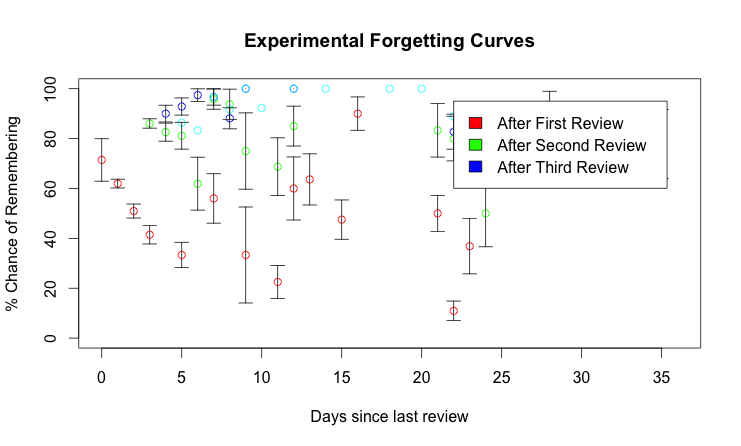
\includegraphics[width=9cm]{img/forgetcurve_5.png}
\caption{Forgetting curves produced from recorded review data with threshold $n \geq 5$}
\label{fig_forgetcurve_5}
\end{figure}

\begin{figure}[h!]
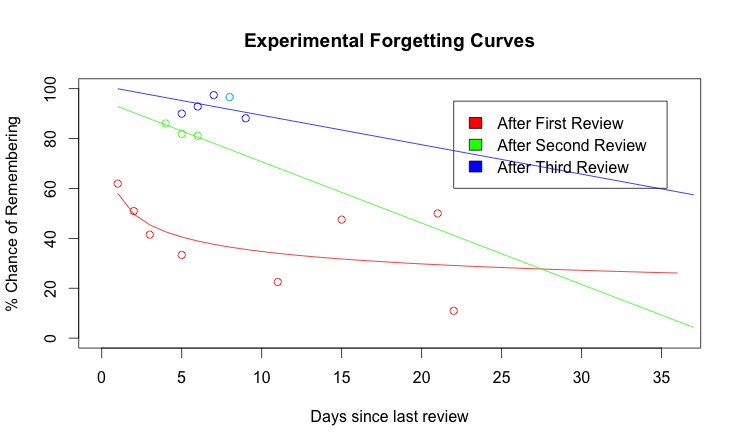
\includegraphics[width=9cm]{img/forgetcurve_30.png}
\caption{Forgetting curves produced from recorded review data with threshold $n \geq 30$}
\label{fig_forgetcurve_30}
\end{figure}

\begin{figure}[h!]
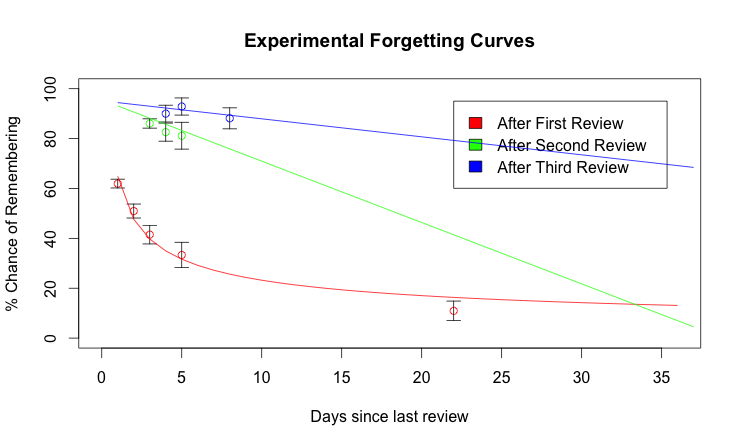
\includegraphics[width=9cm]{img/forgetcurve_50.png}
\caption{Forgetting curves produced from recorded review data with threshold $n \geq 50$}
\label{fig_forgetcurve_50}
\end{figure}

\begin{figure}[h!]
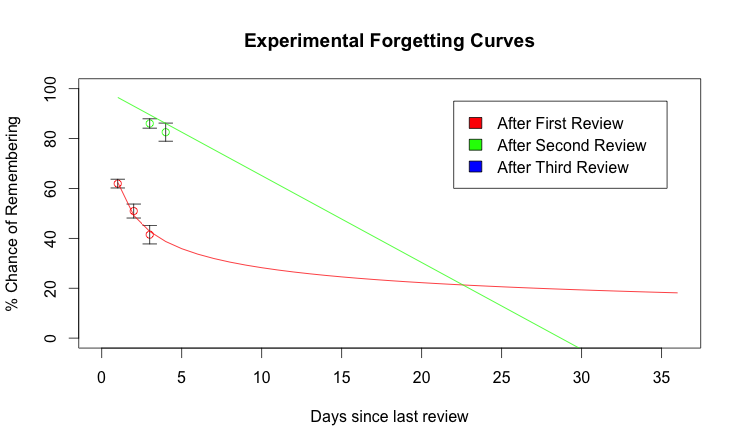
\includegraphics[width=9cm]{img/forgetcurve_100.png}
\caption{Forgetting curves produced from recorded review data with threshold $n \geq 100$}
\label{fig_forgetcurve_100}
\end{figure}


\subsection*{Generated from Machine Learning Algorithms}

\section{Prediction of Recall}


\subsection*{Support Vector Machines}
